\section{Introduction}        
%%问题背景
\subsection{Problem Background}%%二级章节标题
In recent years, under the weight of the domestic shipping market downturn caused by factors such as declining transportation demand, domestic shipping companies have changed their marketing concepts and began to establish e-commerce platforms with dynamic intelligent pricing \parencite{ps} functions for sales \parencite{fp}. The platform can transparently announce different freight prices to customers in real time to achieve the goal of maximizing revenue. 

To match this platform, Shipping Company X plans to develop an intelligent shipping pricing system which can provide timely and accurate pricing strategies to the rapidly changing market, thereby forging an efficient operation system. 

Therefore, it is necessary for Shipping Company X, which has a large number of routes, to design a powerful system that can choose direction flow, study customer booking habits, and formulate pricing strategies. In addition, the dynamic pricing strategy based on big data is more accurate and universal\parencite{dynamic-pricing}.

%%问题重述
\subsection{Clarification and Restatement}
In this problem we are given container transaction data, container information, route data, order information, and existing pricing strategies from July to November 2019, asked to provide the company with a more reasonable pricing strategy for spot market than existing ones.We should only use these data to solve the following problems:
\begin{itemize}
    \item  On the grounds of historical revenue, sales volume, freight rate, region and other factors, select ten suitable flow directions for system testing.
    \item Based on the above screening, the following three issues need to be resolved：
    \begin{itemize}
        \item[-]Research and describe the customer's booking habits in the selected 10 flow directions.
        \item[-]Considering factors such as customer booking habits and macro market changes, launch a research on the relationship between sales and freight.
        \item[-]Forecast the sales volume of one or more selected flow directions.
    \end{itemize}
    \item Choose one of the flow directions to judge the pros and cons of X Ship Company’s existing strategies and provide a more reasonable pricing strategy for the spot market.
    \item Write a memo to the project leader of shipping company X by summarizing the results and strategies.
\end{itemize}

%%工作介绍，简明叙述解题方法和主要成果
\subsection{Our work}
Our work follows the following workflow, as shown in the Figure \ref{fig:workflow}.
\begin{figure}[H]
    \centering
    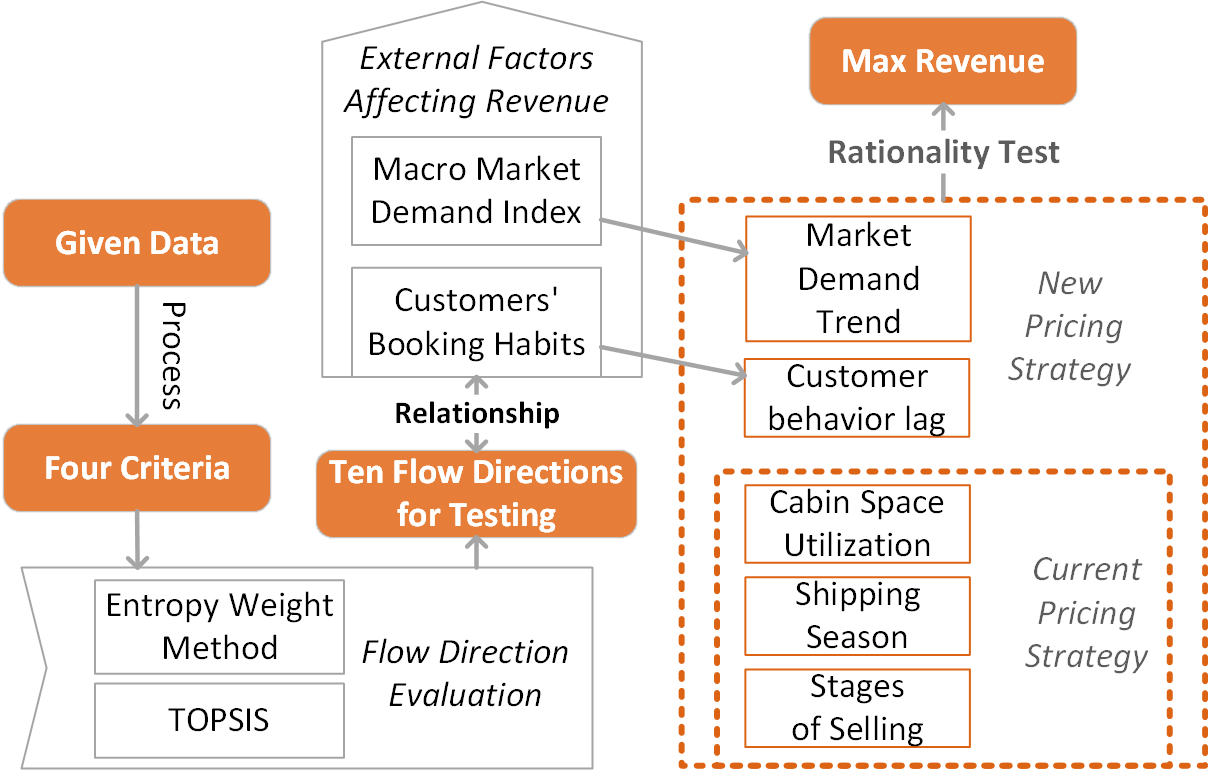
\includegraphics[scale=0.6]{Chapter-Mock/images-Mock/workflow.png}
    \caption{Workflow of Designing Pricing System}
    \label{fig:workflow}
\end{figure}
% We do such things ...
% We begin by establishing a model of ...
\begin{itemize}                %%以圆点方式给出各点
    \item In task 1, we propose four metrics (sales, historical revenue, average freight rate, and port throughput). The Entropy Weight Method is applied to determine the weights. We utilize TOPSIS to implement a comprehensive evaluation and finally select out ten most valuable flow directions for next research.
    \item For task 2(1), we make an analysis on the booking habits of customers. We process the data set to figure out ten violin plots to show the waybill distribution of ten flow directions selected according to the normalized 14-day-long selling period. After that, we apply the algorithm of min-max normalization to discover the evolution trend of the sales volume and the freight rate in one flow direction. We find that customers tend to wait some time after the freight decrease to book the containers.
    \item As to task 2(2), we use Granger Cause Test to study the relationship between the sales volume and the freight rate and get the lag hours related to the former two factors. Additionally, we consider the market demand as an external index and we set a model to calculate it.
    \item As for task 2(3), LSTM is used to predict the market demand index and then to reflect sales volume in short terms. We select three flow directions to make the short-term forecasts and all have satisfactory consequences.
    \item In terms of task 3(1), we make a rationality test to the existing pricing strategy of the shipping company X. We first design a simple pricing strategy to form a basic revenue. Then we simulate the existing pricing strategy, calculate its revenue and define the ratio between these two revenues as the index of rationality.
    \item Regarding task 3(2), we design a new intelligent pricing strategy. We denote a changing rate to control the freight rate change and do the rationality test, which has desired result.
\end{itemize}